\documentclass[12pt,letterpaper]{article}

\usepackage[spanish,es-tabla]{babel}
\usepackage{fontspec}
\IfFontExistsTF{Times New Roman}
  {\setmainfont{Times New Roman}}
  {\setmainfont{TeX Gyre Termes}}
\usepackage{geometry}
\geometry{margin=2.5cm}
\usepackage{setspace}
\onehalfspacing
\usepackage{ragged2e}
\justifying
\usepackage{microtype}
\usepackage{xcolor}
\usepackage{graphicx}
\graphicspath{{imagenes/}{../imagenes/}}
\usepackage{tikz}
\usetikzlibrary{arrows.meta,positioning,shapes.geometric,fit,calc}
\usepackage{booktabs}
\usepackage{array}
\usepackage{tabularx}
\usepackage{float}
\usepackage{caption}
\usepackage{titlesec}
\usepackage{fancyhdr}
\usepackage{xurl}
\usepackage[hidelinks]{hyperref}
\usepackage{adjustbox}
\setlength{\emergencystretch}{3em}

\definecolor{espeGreen}{HTML}{0F3D2E}
\definecolor{deepTeal}{HTML}{123C55}
\definecolor{softGold}{HTML}{C6A24A}
\definecolor{ink}{HTML}{1F2933}
\definecolor{mist}{HTML}{EFF3F1}
\definecolor{cloud}{HTML}{F8FAF8}
\definecolor{accentRed}{HTML}{B44B3F}
\definecolor{steel}{HTML}{44546A}
\definecolor{parchment}{HTML}{D7C79C}
\definecolor{wood}{HTML}{3A271C}
\definecolor{fog}{HTML}{DCE2DE}

\titleformat{\section}{\normalfont\Large\bfseries\color{espeGreen}}{\thesection.}{0.7em}{}
\titleformat{\subsection}{\normalfont\large\bfseries\color{deepTeal}}{\thesubsection.}{0.7em}{}
\captionsetup{font=small,labelfont=bf}

\pagestyle{fancy}
\setlength{\headheight}{14pt}
\fancyhf{}
\lhead{\small BFS en Videojuegos}
\rhead{\small Desarrollo de Videojuegos}
\cfoot{\thepage}
\renewcommand{\headrulewidth}{0.4pt}

\newcolumntype{Y}{>{\RaggedRight\arraybackslash}X}
\newcolumntype{L}[1]{>{\RaggedRight\arraybackslash}p{#1}}

\begin{document}

\thispagestyle{empty}
\begin{tikzpicture}[remember picture,overlay]
  \fill[cloud] (current page.south west) rectangle (current page.north east);
  \fill[espeGreen] (current page.north west) rectangle ([xshift=4.2cm]current page.south west);
  \fill[deepTeal] ([xshift=3.55cm]current page.north west) -- ([xshift=5.05cm]current page.north west) -- ([xshift=3.95cm]current page.south west) -- ([xshift=2.65cm]current page.south west) -- cycle;
  \draw[softGold,line width=1.2pt] ([xshift=13.25cm,yshift=-1.1cm]current page.north west) -- ([xshift=-1.2cm,yshift=-1.1cm]current page.north east);
  \draw[softGold,line width=1.2pt] ([xshift=5.2cm,yshift=1.1cm]current page.south west) -- ([xshift=-1.2cm,yshift=1.1cm]current page.south east);
  \foreach \x/\y/\r in {1.1/-2.0/0.18,2.3/-4.7/0.11,1.5/-7.0/0.14,2.8/-9.6/0.09,1.0/-12.2/0.16,2.6/-15.5/0.12,1.4/-18.0/0.10}{
    \fill[softGold!80] ([xshift=\x cm,yshift=\y cm]current page.north west) circle (\r cm);
  }
  \node[anchor=north west] at ([xshift=5.15cm,yshift=-0.82cm]current page.north west) {
\includegraphics[width=7.9cm]{espe.jpg}};
  \node[anchor=south west,rotate=90,text=cloud!86,font=\Large\bfseries] at ([xshift=1.0cm,yshift=1.7cm]current page.south west) {DESARROLLO DE VIDEOJUEGOS};
  \draw[softGold,line width=0.9pt] ([xshift=0.8cm,yshift=1.35cm]current page.south west) -- ([xshift=0.8cm,yshift=11.5cm]current page.south west);
  \node[anchor=south east,draw=softGold,line width=0.9pt,circle,minimum size=2.2cm,text=espeGreen,font=\Large\bfseries,fill=cloud] at ([xshift=-2.0cm,yshift=1.9cm]current page.south east) {G1};
\end{tikzpicture}

\vspace*{1.65cm}
\noindent\hspace*{4.65cm}
\begin{minipage}{0.66\textwidth}
  \begin{flushleft}
    {\Large\bfseries\color{espeGreen} Universidad de las Fuerzas Armadas ESPE\par}
    \vspace{0.25cm}
    {\large Carrera de Software\par}
    \vspace{0.2cm}
    {\large Desarrollo de Videojuegos\par}
    \vspace{1.55cm}
    {\fontsize{26}{31}\selectfont\bfseries\color{ink} Informe sobre el algoritmo de búsqueda de caminos (BFS) en videojuegos\par}
    \vspace{0.35cm}
    {\Large\color{softGold}\bfseries Proyecto: BFS aplicado a Bad Ice Cream\par}
    \vspace{1.0cm}
    \begin{tikzpicture}
      \draw[softGold,line width=1pt] (0,0) -- (9.7,0);
      \fill[softGold] (0,0) circle (2pt);
      \fill[softGold] (9.7,0) circle (2pt);
    \end{tikzpicture}
    \vspace{0.55cm}

    {\bfseries Grupo:} 1\par
    \vspace{0.25cm}
    {\bfseries Integrantes:}\par
    Jordan Guaman\par
    Mesias Mariscal\par
    Anthony Morales\par
    Denise Rea\par
    \vspace{0.35cm}
    {\bfseries NRC:} 30817\par
    {\bfseries Docente:} Ing. Héctor Pinto\par
    \vspace{0.55cm}
    Sangolquí, Ecuador\par
    Junio de 2026
  \end{flushleft}
\end{minipage}
\clearpage

\tableofcontents
\newpage

\section{Introducción}

Desde los primeros videojuegos en dos dimensiones, el movimiento de los personajes ha sido uno de los problemas centrales del diseño y la programación. Un enemigo que patrulla sin rumbo, un jugador que no sabe hacia dónde ir o un personaje que se queda atascado contra una pared rompen la inmersión y arruinan la experiencia de juego. Para que el movimiento resulte creíble, funcional y coherente con el entorno, los desarrolladores recurren a un conjunto de técnicas conocidas como \textbf{técnicas de movimiento}, dentro de las cuales destaca la \textbf{búsqueda de caminos} (\textit{pathfinding}), una de las ramas más importantes de la inteligencia artificial aplicada a videojuegos.

La búsqueda de caminos consiste en calcular automáticamente una ruta válida —y, en la mayoría de los casos, óptima— entre un punto de origen y un punto de destino dentro de un entorno con obstáculos. Esta disciplina agrupa múltiples algoritmos, cada uno con sus propias ventajas y limitaciones: desde los más sencillos como la búsqueda en anchura (\textit{BFS}) y la búsqueda en profundidad (\textit{DFS}), hasta alternativas más elaboradas como Dijkstra, A*, los Campos de Flujo o las variantes jerárquicas. La elección del algoritmo depende del género del juego, del tamaño del mapa, de la cantidad de agentes en movimiento y de si el terreno presenta costos uniformes o variables.

\begin{figure}[H]
\centering

\includegraphics[width=0.5\textwidth]{bad-ice-cream-presentation.png}
\caption{\textit{Bad Ice Cream} (nitrome, 2010): portada oficial del juego que sirve como caso de estudio para el algoritmo \textit{BFS}.}
\end{figure}

El presente informe se enfoca en uno de esos algoritmos: la búsqueda en anchura (\textit{BFS}, \textit{Breadth-First Search}). Aunque no es el más avanzado, \textit{BFS} destaca por su simplicidad, su optimalidad garantizada en mapas de costos uniformes y su facilidad de implementación, lo que lo convierte en la opción didáctica y técnicamente adecuada para juegos bidimensionales basados en cuadrícula. Para ilustrar su aplicación real, se analiza el caso del videojuego \textit{Bad Ice Cream}, un título de tipo \textit{arcade} de 2010 en el que los enemigos persiguen al jugador a través de un laberinto de bloques de hielo que se crean y destruyen en tiempo real. Este escenario resulta ideal porque el mapa es una cuadrícula discreta, los costos de movimiento son uniformes y los obstáculos cambian constantemente, lo que obliga a recalcular rutas con frecuencia.

El documento se organiza en cuatro ejes: una investigación de las principales técnicas de movimiento y algoritmos de búsqueda de caminos utilizados en la industria, una explicación teórica detallada del algoritmo \textit{BFS}, una descripción de cómo se implementa dentro del motor de un juego y un análisis del caso real de \textit{Bad Ice Cream} donde se identifican los personajes controlados, las situaciones de juego y los beneficios del algoritmo para la jugabilidad.

\section{Objetivos del informe}

\subsection{Objetivo general}

Investigar las técnicas de movimiento aplicadas al desarrollo de videojuegos, exponer el funcionamiento y la aplicación de un algoritmo de búsqueda de caminos, y presentar un juego concreto donde dicho algoritmo se encuentre implementado, tomando como caso de estudio \textit{Bad Ice Cream}.

\subsection{Objetivos específicos}

\begin{itemize}
  \item Investigar y comparar las principales técnicas de movimiento y los algoritmos de búsqueda de caminos empleados en la industria del videojuego, identificando la utilidad y las limitaciones de cada uno.
  \item Explicar de forma detallada el algoritmo \textit{BFS}: su objetivo, el manejo de nodos y costos, el tratamiento de obstáculos, los pasos de ejecución, la reconstrucción de la ruta final y sus limitaciones.
  \item Describir cómo se implementa \textit{BFS} dentro del motor de un juego: representación del mapa, definición del origen y el destino, manejo de obstáculos dinámicos, ciclo de cálculo y seguimiento de la ruta por parte del personaje.
  \item Analizar el caso del videojuego \textit{Bad Ice Cream}, identificando los personajes controlados por la IA, las situaciones de juego y el beneficio concreto que \textit{BFS} aporta a la jugabilidad.
\end{itemize}

\section{Técnicas de búsqueda de caminos en videojuegos}

La búsqueda de caminos no es un problema único: existen múltiples algoritmos que priorizan distintos criterios, como la optimalidad de la ruta, el uso de memoria o la velocidad de respuesta ante mapas que cambian. Elegir el algoritmo correcto depende del género del juego, del tamaño del mapa, de la cantidad de agentes que se mueven y de si el terreno es uniforme o tiene distintos costos de tránsito.

\begin{table}[H]
\centering
\caption{Técnicas de búsqueda de caminos y su utilidad en videojuegos}
\small
\begin{tabularx}{\textwidth}{L{4.0cm}Y}
\toprule
\textbf{Técnica} & \textbf{Descripción y utilidad en videojuegos} \\
\midrule
A* (A-Estrella) &
Combina el costo real recorrido con una estimación heurística hacia la meta. Es el estándar de la industria; se utiliza en \textit{RTS}, \textit{MOBAs} y \textit{RPGs} para un movimiento preciso y eficiente al hacer clic sobre el terreno. \\
\addlinespace
Dijkstra &
Explora en todas las direcciones calculando el costo real hacia cada nodo posible, sin usar heurísticas. Es ideal cuando se busca el punto de interés más cercano (por ejemplo, un botiquín o una zona de cobertura) en lugar de un destino único. \\
\addlinespace
Búsqueda en Anchura (BFS) &
Se expande en forma de anillos concéntricos, asumiendo que todos los movimientos tienen el mismo costo. Es excelente para mapas de cuadrícula, como en los juegos de rol tácticos por turnos, para mostrar el área de movimiento posible. \\
\addlinespace
Búsqueda en Profundidad (DFS) &
Avanza lo más lejos posible por una ruta y retrocede si encuentra un callejón sin salida. No se usa para mover personajes; su fuerte es la generación procedimental y la verificación de laberintos. \\
\addlinespace
D* y LPA* &
Variantes avanzadas de A* que almacenan cálculos previos para adaptarse a cambios sin reiniciar. Son indispensables en entornos dinámicos y destructibles donde los obstáculos cambian repentinamente en medio del camino. \\
\addlinespace
Puntos de Salto (JPS) &
Optimización matemática de A* que se salta nodos vacíos y busca directamente cambios de dirección forzados. Es fundamental en simuladores y \textit{RTS} a gran escala para mover miles de unidades simultáneamente sin saturar la CPU. \\
\addlinespace
Voraz el Mejor Primero &
Ignora el costo recorrido y se guía exclusivamente por la estimación visual hacia el objetivo. Es perfecto para hordas de enemigos "tontos" y agresivos (como zombis) que persiguen al jugador sin buscar la ruta perfecta. \\
\addlinespace
Theta* &
Permite el cálculo de trayectorias en línea recta entre dos puntos si no hay obstáculos en medio. Se usa en juegos modernos 3D y mundos abiertos para evitar movimientos robóticos en zigzag sobre cuadrículas invisibles. \\
\addlinespace
Jerárquico A* (HPA*) &
Divide un mapa gigante en áreas más pequeñas y calcula rutas abstractas de un área a otra antes del detalle. Es crucial en juegos de mundo abierto (\textit{MMORPGs}) para que la IA planee viajes largos sin consumir enormes cantidades de memoria. \\
\addlinespace
Campos de Flujo &
Asigna un vector direccional a cada celda del mapa, guiando el movimiento como si fuera una corriente. Es la solución definitiva para juegos con enjambres masivos, permitiendo a cientos de unidades navegar sin calcular cientos de rutas individuales. \\
\bottomrule
\end{tabularx}
\end{table}

De la tabla anterior se observa que \textit{BFS} no es el algoritmo más avanzado ni el más eficiente en mapas grandes, pero sí es el más sencillo de implementar y el más confiable cuando el terreno es uniforme y el mapa se representa como una matriz discreta. Esa es la razón por la que resulta perfecto para juegos como \textit{Bad Ice Cream}, donde el escenario es una cuadrícula, los costos de movimiento son iguales para todas las celdas y los enemigos necesitan recalcular su ruta cada vez que el jugador modifica el entorno.

\section{Explicación del algoritmo BFS}

\subsection{Objetivo del algoritmo}

El objetivo principal de \textit{BFS} es encontrar el camino más corto garantizado entre un punto de origen y un destino dentro de un grafo no ponderado, como por ejemplo una cuadrícula plana. Su filosofía es explorar el entorno por "capas" o "anillos concéntricos": primero revisa todos los lugares que están a un paso de distancia, después los que están a dos pasos, y así sucesivamente, hasta localizar el destino.

\subsection{Los nodos}

En el contexto de un videojuego en 2D, el mapa se divide en una cuadrícula (matriz).

\begin{itemize}
  \item Cada celda o casilla de esa cuadrícula es un \textbf{nodo}.
  \item Cada nodo almacena información vital: sus coordenadas $(x, y)$, su estado (\textit{transitable} o \textit{no transitable}) y, durante la ejecución del algoritmo, un puntero hacia su \textbf{nodo padre}, es decir, la casilla desde la cual el algoritmo llegó a él.
\end{itemize}

\subsection{Los costos}

A diferencia del algoritmo de Dijkstra o de A*, \textit{BFS} no maneja costos variables.

\begin{itemize}
  \item Asume que moverse a cualquier nodo vecino cuesta exactamente lo mismo, es decir, \textbf{costo = 1}.
  \item No distingue entre caminar por asfalto, lodo o agua. Por esta razón, solo es útil en juegos donde el terreno es uniforme y el único factor que importa es la cantidad de pasos (o casillas) para llegar al objetivo.
\end{itemize}

\subsection{Los obstáculos}

Los obstáculos (paredes, bloques de hielo, enemigos) son simplemente nodos marcados lógicamente como \textit{no transitables} o bloqueados. Cuando el algoritmo evalúa los nodos vecinos para expandirse, verifica esta propiedad: si el nodo es un obstáculo, lo descarta de inmediato y no lo añade a su lista de exploración. Esto obliga al "anillo de búsqueda" a rodear el bloqueo y continuar la exploración por los caminos válidos.

\subsection{Pasos de ejecución (el motor lógico)}

Para implementarlo, \textit{BFS} utiliza una estructura de datos llamada \textbf{Cola} (\textit{Queue}), que funciona bajo el principio \textit{FIFO} (\textit{First In, First Out}: el primero en entrar es el primero en salir). El algoritmo sigue esta secuencia:

\begin{enumerate}
  \item \textbf{Inicialización:} se crea la Cola de exploración y una lista de nodos \textit{Visitados}, cuyo propósito es no procesar la misma casilla dos veces.
  \item \textbf{Arranque:} se toma el nodo de Origen, se marca como \textit{Visitado} y se encola.
  \item \textbf{Ciclo de búsqueda:} mientras la Cola no esté vacía, se desencola (extrae) el primer nodo.
  \item \textbf{Validación de destino:} si el nodo extraído es el Destino, el algoritmo se detiene (es un éxito).
  \item \textbf{Expansión:} si no es el destino, el algoritmo revisa sus nodos vecinos inmediatos: arriba, abajo, izquierda y derecha.
  \item \textbf{Encolado:} por cada vecino que sea transitable y que no haya sido visitado antes:
  \begin{itemize}
    \item Se marca como \textit{Visitado}.
    \item Se guarda el nodo actual como su \textit{padre}.
    \item Se añade al final de la Cola.
  \end{itemize}
  \item El ciclo se repite desde el paso 3.
\end{enumerate}

\subsection{La ruta final (backtracking)}

Una vez que el algoritmo "toca" el nodo Destino en el paso 4, la búsqueda termina, pero aún no se tiene la ruta completa. Para reconstruirla, se realiza un proceso de \textbf{rastreo inverso}:

\begin{enumerate}
  \item El algoritmo toma el nodo Destino y lee quién es su nodo padre.
  \item Salta a ese padre y lee al abuelo, luego al bisabuelo, y así sucesivamente.
  \item Continúa este rastreo hacia atrás hasta llegar al nodo de Origen.
  \item Finalmente, invierte esta lista de nodos, entregando al personaje la secuencia exacta de pasos hacia adelante para llegar a la meta.
\end{enumerate}

\subsection{Limitaciones}

Es importante mencionar por qué \textit{BFS} no se utiliza en todos los juegos:

\begin{itemize}
  \item \textbf{Alto consumo de memoria (RAM):} al expandirse en todas las direcciones de forma indiscriminada (como una gota de agua cayendo en un charco), guarda demasiados nodos inútiles en la memoria antes de encontrar el destino.
  \item \textbf{Ceguera direccional (sin heurística):} no sabe hacia dónde está la meta. Si el destino está a la derecha, \textit{BFS} igual perderá tiempo explorando a la izquierda, arriba y abajo.
  \item \textbf{Inútil en terrenos complejos:} como no evalúa costos, si hay un camino corto pero lleno de lava y un camino ligeramente más largo pero seguro, \textit{BFS} elegirá ciegamente el de la lava por tener menos pasos.
\end{itemize}

\section{Aplicación práctica del algoritmo en un motor de juego}

En el desarrollo de un juego como \textit{Bad Ice Cream}, el algoritmo no flota en el aire: interactúa directamente con la estructura de datos del motor. A continuación se describe cómo funciona \textit{BFS} "bajo el capó".

\subsection{El mapa: tilemap y matrices}

El escenario completo no es más que una matriz bidimensional (un \textit{array} 2D) en la memoria del juego. Cada fruta, muro de hielo o espacio vacío ocupa una celda exacta, por ejemplo \texttt{mapa[x][y]}. Esto simplifica enormemente el entorno para el algoritmo, ya que convierte un mundo gráfico en un grafo matemático perfecto.

% En subsection "El mapa: tilemap y matrices"
\begin{figure}[H]
\centering
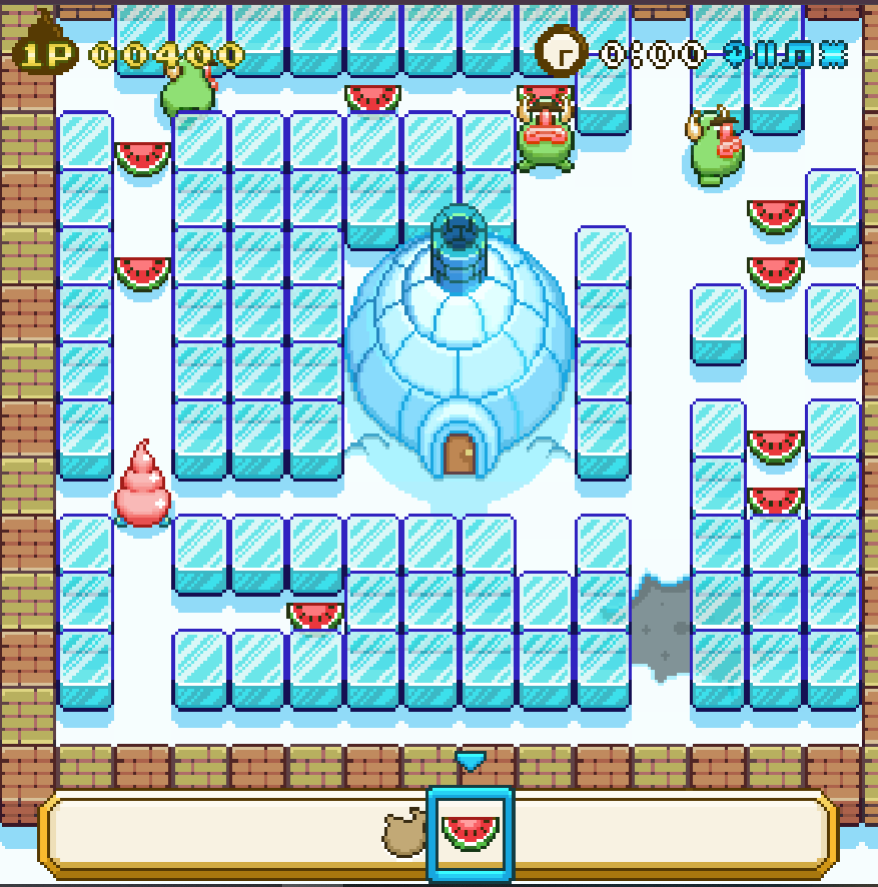
\includegraphics[width=0.5\textwidth]{bad-ice-cream3.png}
\caption{Cuadrícula completa de \textit{Bad Ice Cream}: el escenario se modela como una matriz \texttt{mapa[x][y]} donde cada celda es un nodo para \textit{BFS}.}
\end{figure}

\subsection{Origen y destino}

\begin{itemize}
  \item El \textbf{Origen} se actualiza constantemente y corresponde a las coordenadas actuales en la matriz del enemigo (por ejemplo, la Vaca o el Monstruo Verde).
  \item El \textbf{Destino} son las coordenadas dinámicas del jugador, es decir, el helado que el enemigo intenta atrapar.
\end{itemize}

\subsection{Obstáculos estáticos y dinámicos}

A nivel lógico, una celda vacía tiene un valor de \texttt{0} (transitable) y un bloque de hielo tiene un valor de \texttt{1} (no transitable). La particularidad de este juego es que el mapa \textbf{muta en tiempo real}: cuando el jugador dispara su habilidad, cambia los valores de la matriz de \texttt{0} a \texttt{1} (creando hielo) o de \texttt{1} a \texttt{0} (rompiendo hielo). Esta naturaleza dinámica obliga a recalcular las rutas de los enemigos constantemente.

\begin{figure}[H]
\centering
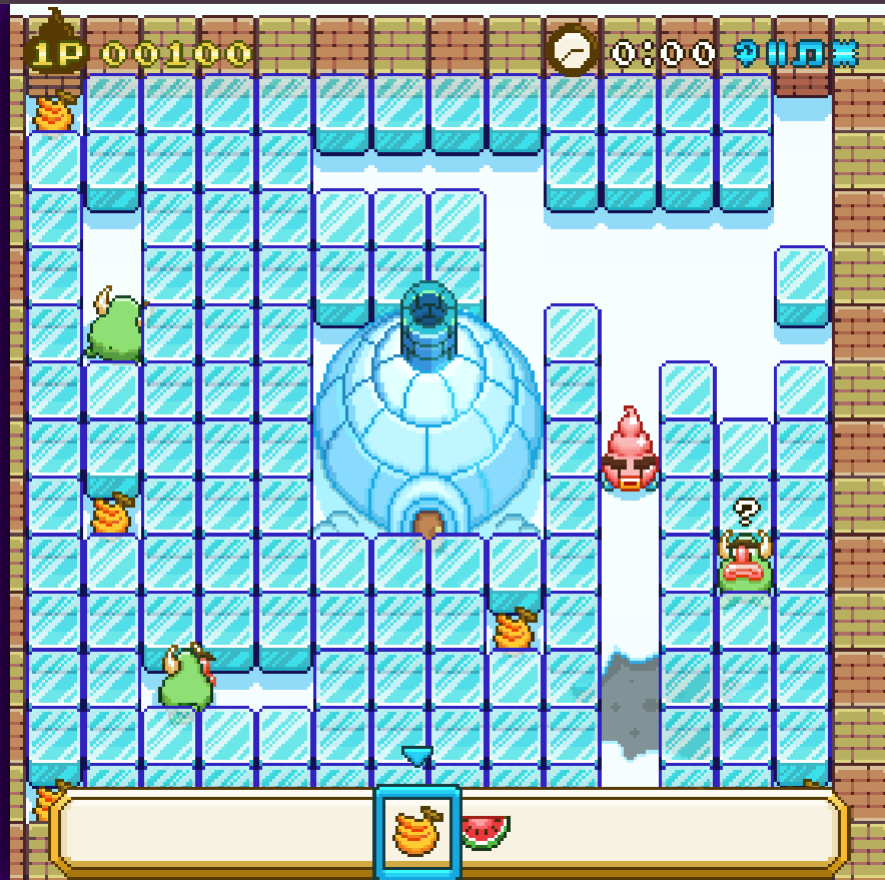
\includegraphics[width=0.5\textwidth]{bad-ice-cream2.png}
\caption{Obstáculos dinámicos: el jugador rompe bloques de hielo (cambiando celdas de \texttt{1} a \texttt{0}), lo que obliga a la IA a recalcular la ruta con \textit{BFS}.}
\end{figure}

\subsection{Cálculo: el game loop y la cola FIFO}

\begin{itemize}
  \item Para no saturar el procesador, \textit{BFS} no se calcula en cada fotograma (\textit{frame}), sino a través de eventos (\textit{event-driven}): se recalcula cada vez que el mapa cambia (cuando el jugador crea o rompe hielo) o cuando el enemigo termina de moverse a una casilla.
  \item El algoritmo utiliza una estructura de datos de Cola (\textit{FIFO - First In, First Out}). Inserta la posición del enemigo y comienza a encolar las casillas vecinas (Norte, Sur, Este, Oeste) que tengan valor \texttt{0}, descartando las que tengan valor \texttt{1}. Se expande en forma de onda hasta que las coordenadas evaluadas coincidan con las del jugador.
\end{itemize}

\subsection{Seguimiento de ruta (path following)}

Una vez que \textit{BFS} alcanza al jugador, realiza un rastreo inverso a través de los nodos padre para construir un arreglo (array) unidimensional con los pasos exactos, por ejemplo \texttt{[Arriba, Arriba, Izquierda, Abajo]}. El script de movimiento del enemigo simplemente lee el primer elemento de ese arreglo, mueve el \textit{sprite} gráficamente a esa celda, lo elimina del arreglo y pasa al siguiente elemento. De esta forma, el enemigo avanza casilla por casilla siguiendo la ruta calculada.

\section{Caso de estudio: BFS en el videojuego Bad Ice Cream}

\subsection{Personaje analizado}

El \textbf{personaje analizado} son los enemigos controlados por la IA (\textit{Inteligencia Artificial}). En los primeros niveles, algunos monstruos solo patrullan de forma aleatoria, pero los enemigos avanzados entran en un estado de \textbf{persecución activa} donde entra en juego el algoritmo \textit{BFS}. Estos enemigos son los responsables de dar tensión al juego, ya que están diseñados para alcanzar al jugador a través del laberinto, sin importar cuántas paredes de hielo se coloquen en su camino.

% En subsection "Personaje analizado"
\begin{figure}[H]
\centering
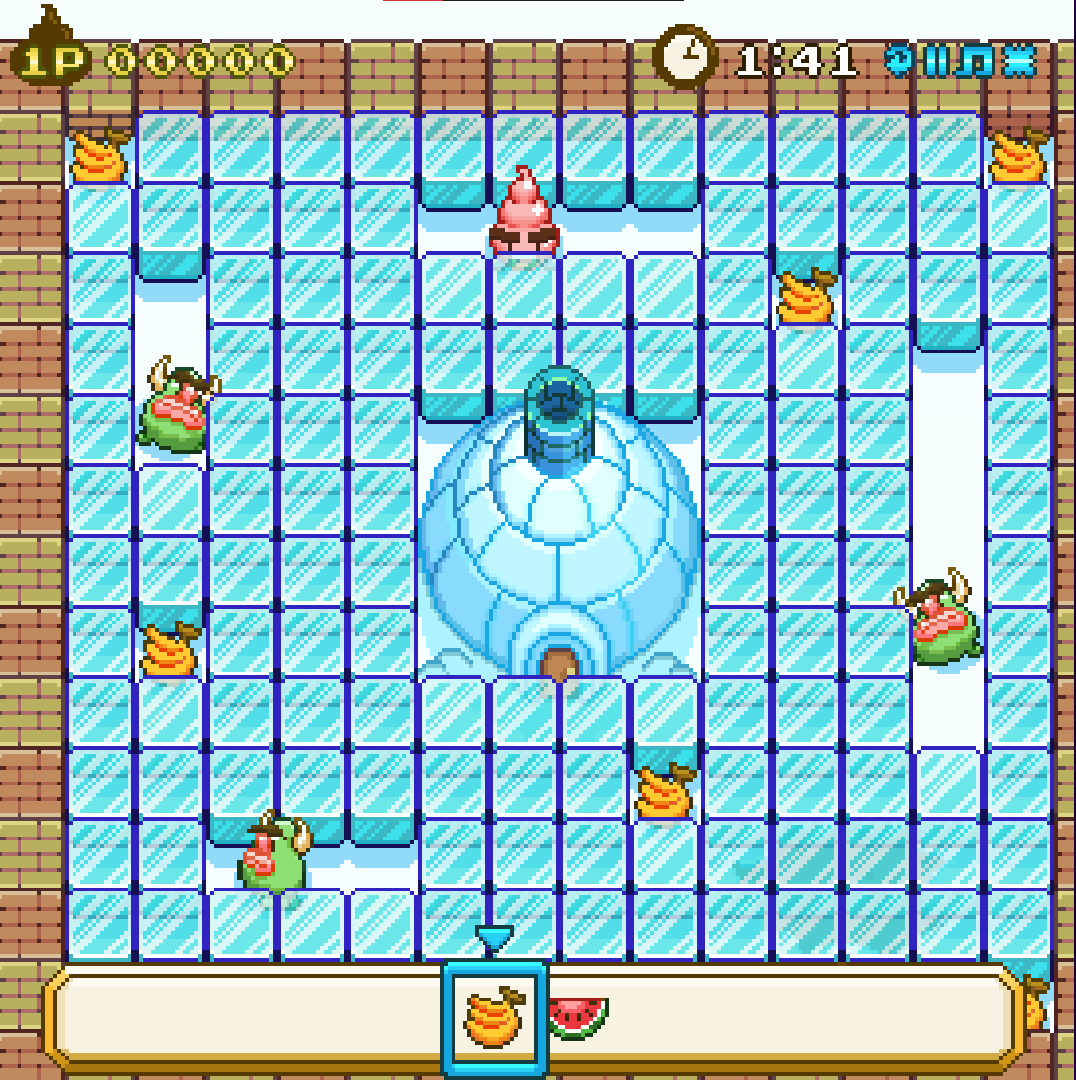
\includegraphics[width=0.55\textwidth]{bad-ice-cream.png}
\caption{Personajes controlados por la IA: los enemigos \textit{slime} persiguen al helado activando el modo de persecución mediante \textit{BFS}.}
\end{figure}

\subsection{Situación de juego (core loop)}

La mecánica principal (\textit{core mechanic}) de \textit{Bad Ice Cream} es el \textbf{control del espacio}. El jugador está atrapado en una arena cerrada recogiendo frutas, y su única defensa es alterar la arquitectura del laberinto construyendo o destruyendo paredes de hielo, ya sea para encerrar a los enemigos o para abrirse paso y escapar. Cada decisión espacial del jugador modifica la matriz del mapa, lo que obliga a la IA a recalcular su ruta de inmediato.

% En subsection "Situación de juego (core loop)"
\begin{figure}[H]
\centering
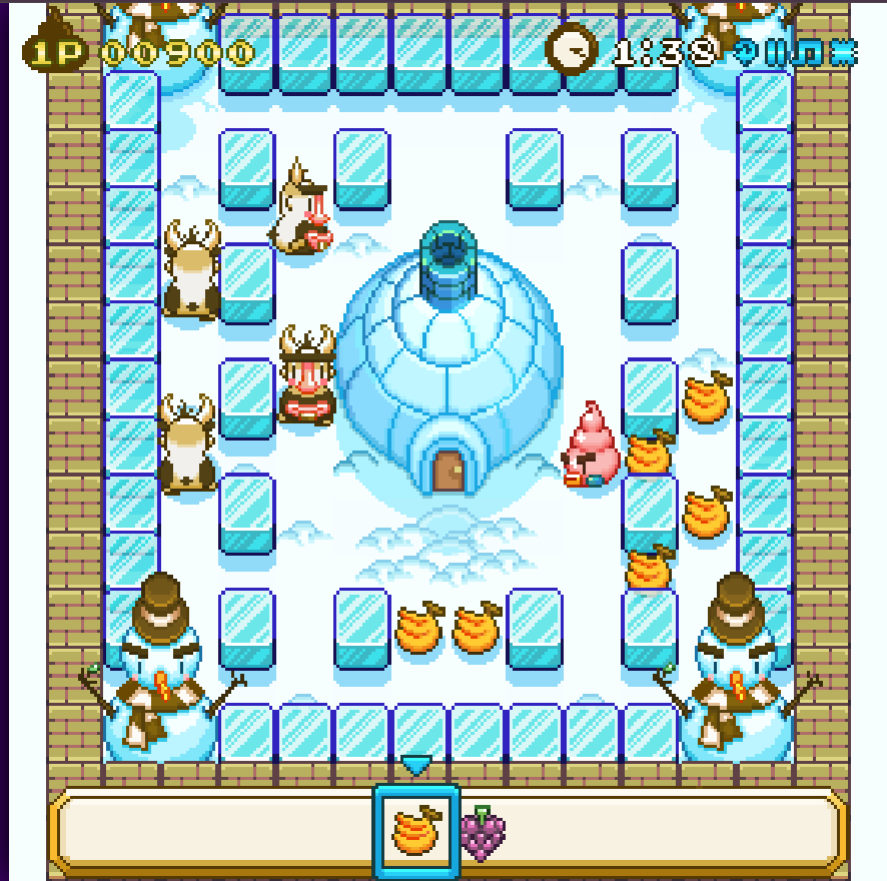
\includegraphics[width=0.55\textwidth]{bad-ice-cream4.png}
\caption{Core loop: el jugador modifica el laberinto de hielo mientras múltiples tipos de enemigos (yetis, cascos, fuego) lo persiguen.}
\end{figure}

\subsection{Beneficio del algoritmo para la jugabilidad}

El uso de \textit{BFS} en \textit{Bad Ice Cream} aporta dos beneficios claros a la experiencia de juego:

\begin{itemize}
  \item \textbf{Evita el "Queso" (Cheesing):} en diseño de videojuegos, \textit{cheesear} significa usar un truco barato para ganar sin esfuerzo. Si los enemigos no tuvieran \textit{BFS} y solo caminaran hacia el jugador en línea recta, el jugador podría simplemente poner un bloque de hielo frente a ellos y quedarse quieto recogiendo frutas, mientras el enemigo choca infinitamente contra el hielo. \textit{BFS} elimina esta estrategia porque el enemigo siempre busca un camino alternativo.
  \item \textbf{Presión constante:} gracias a \textit{BFS}, en el instante en que el jugador coloca un muro de hielo, la matriz se actualiza y la IA percibe que su camino actual está bloqueado. El algoritmo ejecuta una nueva búsqueda en anchura, encuentra el pasillo lateral más cercano y flanquea al jugador. Esto obliga al jugador a estar en constante movimiento y a pensar rápido, creando la dificultad y el valor de entretenimiento reales del juego.
\end{itemize}

% En subsection "Beneficio del algoritmo para la jugabilidad"
\begin{figure}[H]
\centering
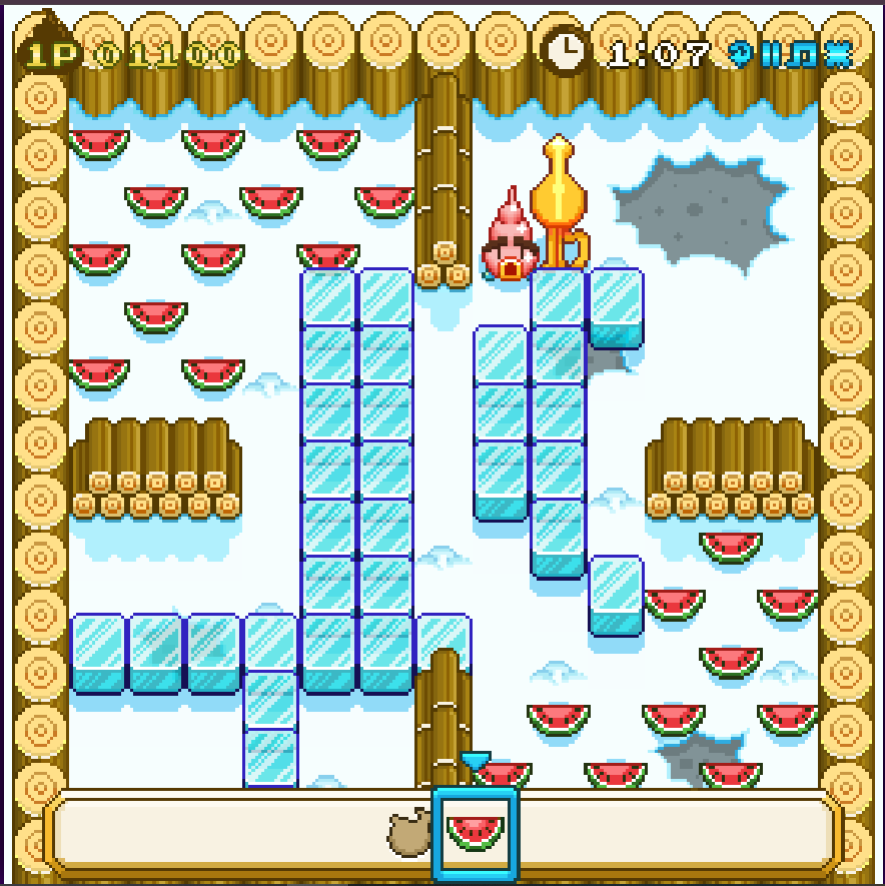
\includegraphics[width=0.55\textwidth]{bad-ice-cream5.png}
\caption{Presión constante: el enemigo de fuego navega una estructura compleja de paredes de hielo, rodeando los muros para alcanzar al jugador.}
\end{figure}

\section{Flujo de ejecución y comparación del algoritmo BFS}

\subsection{Flujo de ejecución}

El siguiente diagrama resume el flujo lógico que sigue \textit{BFS} desde su inicialización hasta la reconstrucción de la ruta final mediante \textit{backtracking}.

\begin{figure}[H]
\centering
\begin{adjustbox}{max width=\textwidth, max height=0.82\textheight, center}
\begin{tikzpicture}[
  node distance=0.45cm and 1.1cm,
  every node/.style={font=\small, align=center},
  start/.style={draw=espeGreen,rounded corners=3pt,fill=espeGreen!15,minimum width=3cm,minimum height=0.55cm},
  process/.style={draw=deepTeal,rounded corners=3pt,fill=mist,minimum width=3cm,minimum height=0.55cm},
  decision/.style={draw=softGold,rounded corners=3pt,fill=softGold!20,diamond,aspect=2.5,inner sep=1pt,minimum width=2.4cm},
  success/.style={draw=espeGreen,rounded corners=3pt,fill=espeGreen!25,minimum width=3cm,minimum height=0.55cm},
  fail/.style={draw=accentRed,rounded corners=3pt,fill=accentRed!15,minimum width=3cm,minimum height=0.55cm},
  arrow/.style={-{Latex[length=2mm]},line width=0.6pt,color=steel}
]
% Columna izquierda: inicialización
\node[start] (ini) {Inicio};
\node[process,below=of ini] (init) {Inicializar Cola\\y Visitados};
\node[process,below=of init] (mark) {Marcar Origen\\y encolar};

% Columna derecha: bucle principal (desplazada a la derecha y abajo)
\node[decision,right=1.2cm of mark,yshift=-0.3cm] (empty) {¿Cola vacía?};
\node[fail,right=of empty] (noroute) {Fin: sin ruta};
\node[process,below=of empty] (deq) {Desencolar nodo};
\node[decision,below=of deq] (target) {¿Es el Destino?};
\node[success,right=of target] (back) {Backtracking\\y Fin};
\node[process,below=of target] (expand) {Expandir vecinos (N, S, E, O)};
\node[process,below=of expand] (enq) {Por cada vecino válido:\\marcar, padre, encolar};

% Conexiones
\draw[arrow] (ini) -- (init);
\draw[arrow] (init) -- (mark);
\draw[arrow] (mark) -- (mark -| empty) node[midway,above,font=\scriptsize]{};
\draw[arrow] (mark -| empty) -- (empty);
\draw[arrow] (empty) -- node[above,font=\scriptsize]{Sí} (noroute);
\draw[arrow] (empty) -- node[right,font=\scriptsize]{No} (deq);
\draw[arrow] (deq) -- (target);
\draw[arrow] (target) -- node[above,font=\scriptsize]{Sí} (back);
\draw[arrow] (target) -- node[right,font=\scriptsize]{No} (expand);
\draw[arrow] (expand) -- (enq);
\draw[arrow] (enq.west) -- ++(-1.3cm,0) |- (deq.west);
\end{tikzpicture}
\end{adjustbox}
\caption{Flujo de ejecución del algoritmo \textit{BFS}: inicialización (izquierda) y bucle principal (derecha) con retorno al desencolar.}
\end{figure}

\subsection{Comparación con otros algoritmos}

Para situar a \textit{BFS} frente a sus alternativas más comunes, la siguiente tabla resume sus características frente a Dijkstra y A*.

\begin{table}[H]
\centering
\caption{Comparación entre BFS, Dijkstra y A*}
\small
\begin{tabularx}{\textwidth}{L{2.4cm}L{3.0cm}L{3.6cm}Y}
\toprule
\textbf{Criterio} & \textbf{BFS} & \textbf{Dijkstra} & \textbf{A*} \\
\midrule
Tipo de grafo & No ponderado & Ponderado (costos $\geq 0$) & Ponderado con heurística. \\
Usa heurística & No & No & Sí. \\
Camino más corto & Sí (en pasos) & Sí (en costo) & Sí (si la heurística es admisible). \\
Complejidad temporal & $O(V + E)$ & $O((V + E)\log V)$ & $O((V + E)\log V)$ en el mejor caso. \\
Consumo de memoria & Alto en mapas grandes & Alto en mapas grandes & Menor que BFS gracias a la heurística. \\
Terreno uniforme & Ideal & No aporta ventaja & No aporta ventaja. \\
Terreno con costos & No recomendado & Ideal & Ideal. \\
Mapa cambiante & Recalcula completo & Recalcula completo & Recalcula; mejor con D*/LPA*. \\
Caso ideal & \textit{Bad Ice Cream}, juegos por turnos. & Botiquín más cercano, cobertura. & Movimiento con clic en \textit{RTS}/\textit{RPGs}. \\
\bottomrule
\end{tabularx}
\end{table}

La tabla anterior confirma que \textit{BFS} no compite en mapas grandes con costos variables, pero sigue siendo la elección natural en el nicho específico de los juegos bidimensionales de cuadrícula con terreno uniforme y obstáculos que cambian a alta frecuencia, como es el caso de \textit{Bad Ice Cream}.

\section{Conclusiones}

El análisis realizado confirma que el algoritmo de búsqueda en anchura (\textit{BFS}) es una herramienta fundamental dentro del desarrollo de videojuegos bidimensionales, no por ser el más sofisticado, sino por ser el más adecuado cuando el mapa se representa como una cuadrícula de costos uniformes.

En primer lugar, la investigación de las distintas técnicas de búsqueda de caminos permitió identificar el nicho exacto donde \textit{BFS} ofrece su mayor ventaja: mapas de cuadrícula pequeños o medianos con terreno homogéneo, donde se necesita un camino óptimo en pasos y no en costo variable. Frente a algoritmos más avanzados como A*, JPS o los Campos de Flujo, \textit{BFS} se posiciona como la opción más simple, más fácil de implementar y suficiente para juegos de tipo \textit{arcade}.

En segundo lugar, la explicación teórica del algoritmo demostró que su lógica es elegante y compacta: inicializar, encolar, expandir en capas y reconstruir con \textit{backtracking}. Sin embargo, también quedaron claras sus limitaciones: alto consumo de memoria en mapas grandes, ausencia de heurística que guíe la búsqueda y ceguera frente a terrenos con distintos costos. Estas limitaciones explican por qué la industria reserva \textit{BFS} para casos muy concretos, como los juegos por turnos y los \textit{arcade} de cuadrícula.

En tercer lugar, la aplicación práctica en el motor del juego evidenció que la potencia de \textit{BFS} no está solo en encontrar la ruta, sino en poder recalcularla de manera continua. En \textit{Bad Ice Cream}, el mapa muta cada vez que el jugador dispara su poder, y aun así el algoritmo responde con suficiente rapidez para mantener la persecución fluida. La estructura de Cola (\textit{FIFO}) encaja perfectamente con un motor basado en eventos (\textit{event-driven}) y permite que cada enemigo tenga su propia ruta independiente.

Finalmente, el caso de estudio de \textit{Bad Ice Cream} validó la utilidad de \textit{BFS} para la jugabilidad. Sin \textit{BFS}, los enemigos podrían ser "engañados" fácilmente colocando un bloque de hielo; con \textit{BFS}, el enemigo siempre encuentra un camino alternativo, lo que elimina el \textit{cheese} y genera la presión constante que da sentido al reto del juego. Se concluye entonces que, para proyectos de desarrollo de videojuegos con mecánicas similares, \textit{BFS} sigue siendo una solución vigente, didáctica y perfectamente funcional.

\end{document}
